\section{Background}
This chapter provides the requisite background information for understanding the concepts and techniques utilized in our enhanced quantum implementation for uniform random sampling in software product lines (SPLs).
It covers the necessary fundamentals of SPLs, quantum computing principles, and Grover's algorithm. 
This background chapter will only explain the knowledge needed to understand the improvement implemented and proposed by this paper.

\begin{figure*}
    \centering
    \usetikzlibrary{angles}
\usetikzlibrary{positioning}
\definecolor{drawColor}{RGB}{128 128 128}
\newcommand{\circleSize}{0.25em}
\newcommand{\angleSize}{0.8em}

\forestset{
	/tikz/mandatory/.style={
		circle,fill=drawColor,
		draw=drawColor,
		inner sep=\circleSize
	},
	/tikz/optional/.style={
		circle,
		fill=white,
		draw=drawColor,
		inner sep=\circleSize
	},
	featureDiagram/.style={
		for tree={
			minimum height = 0.6cm,
			text depth = 0,
			draw = drawColor,
			edge = {draw=drawColor},
			parent anchor = south,
			child anchor = north,
			l sep = 2em,
			s sep = 1em,
		}
	},
	/tikz/redColor/.style={
		fill = red!60,
		draw = drawColor
	},
	/tikz/orangeColor/.style={
		fill = orange!50,
		draw = drawColor
	},
	/tikz/yellowColor/.style={
		fill = yellow!50,
		draw = drawColor
	},
	/tikz/darkGreenColor/.style={
		fill = black!30!green,
		draw = drawColor
	},
	/tikz/lightGreenColor/.style={
		fill = green!30,
		draw = drawColor
	},
	/tikz/cyanColor/.style={
		fill = cyan!30,
		draw = drawColor
	},
	/tikz/lightGrayColor/.style={
		fill = black!10,
		draw = drawColor
	},
	/tikz/blueColor/.style={
		fill = blue!50,
		draw = drawColor
	},
	/tikz/magentaColor/.style={
		fill = magenta,
		draw = drawColor
	},
	/tikz/pinkColor/.style={
		fill = pink!90,
		draw = drawColor
	},
	/tikz/abstract/.style={
		fill = blue!85!cyan!5,
		draw = drawColor
	},
	/tikz/concrete/.style={
		fill = blue!85!cyan!20,
		draw = drawColor
	},
	mandatory/.style={
		edge label={node [mandatory] {} }
	},
	optional/.style={
		edge label={node [optional] {} }
	},
	or/.style={
		tikz+={
			\path (.parent) coordinate (A) -- (!u.children) coordinate (B) -- (!ul.parent) coordinate (C) pic[fill=drawColor, angle radius=\angleSize]{angle};
		}	
	},
	/tikz/or/.style={
	},
	alternative/.style={
		tikz+={
			\path (.parent) coordinate (A) -- (!u.children) coordinate (B) -- (!ul.parent) coordinate (C) pic[draw=drawColor, angle radius=\angleSize]{angle};
		}	
	},
	/tikz/alternative/.style={
	},
	/tikz/placeholder/.style={
	},
	collapsed/.style={
		rounded corners,
		no edge,
		for tree={
			fill opacity=0,
			draw opacity=0,
			l = 0em,
		}
	},
	/tikz/hiddenNodes/.style={
		midway,
		rounded corners,
		draw=drawColor,
		fill=white,
		minimum size = 1.2em,
		minimum width = 0.8em,
		scale=0.9
	},
}

\begin{forest}
	featureDiagram
	[Sandwich,concrete[Bread,concrete,mandatory[Full Grain ,concrete,alternative][Toast,concrete][Flatbread,concrete]][Cheese,concrete,optional[Gouda,concrete,optional][Cheddar,concrete,optional]][Meat,concrete,optional[Salami ,concrete,optional][Ham,concrete,optional]]]	
	\matrix [anchor=north west] at (current bounding box.north east) {
		\node [placeholder] {}; \\
	};
	\matrix [draw=drawColor,anchor=north west] at (current bounding box.north east) {
		\node [label=center:\underline{Legend:}] {}; \\
		\node [concrete,label=right:Feature] {}; \\
		\node [mandatory,label=right:Mandatory] {}; \\
		\node [optional,label=right:Optional] {}; \\
			\draw[drawColor] (0.1,0) -- +(-0.2, -0.4);
			\draw[drawColor] (0.1,0) -- +(0.2,-0.4);
			\draw[drawColor] (0,-0.2) arc (240:300:0.2);
		\node [alternative,label=right:Alternative Group] {}; \\	};
	\matrix [below=1mm of current bounding box] {
	\node {\( \text{Full Grain } \Rightarrow \text{Gouda} \land \text{Salami } \)}; \\
	\node {\( \text{Toast} \Rightarrow \text{Gouda} \land \text{Salami } \)}; \\
	};
\end{forest}
    \caption{Feature Model describing a Sandwich with additional constraints.}
    \label{fig:bg:spl:sandwich-imply-model}
\end{figure*}

\subsection{Software Product Lines}
A software product line (SPL) represents a strategic approach to software engineering that prioritizes the systematic production of a family of related software products \cite{spl-pohl, KCHNP:TR90}.
In contrast to the development of each product from its inception, SPLs prioritize the reuse of fundamental assets, including code, designs, and documentation, across a range of products \cite{ClementsSoftwareProduct2001}.
This methodology is particularly advantageous in domains where products exhibit a shared set of characteristics while necessitating adaptations for diverse markets, customer requirements, or operational contexts.
SPLs endeavor to enhance productivity, expedite time-to-market, and elevate product quality by capitalizing on this common ground while navigating the inherent variability.

In the context of software product lines, constraints are defined as rules or conditions that dictate the valid combinations of features within a given product configuration. 
These constraints guarantee that the selected features are compatible and that the resulting product adheres to the intended design and functionality. 
Constraints may be expressed in a number of ways, including as mandatory features, mutual exclusions (where the inclusion of one feature precludes the inclusion of another), or dependencies (where the inclusion of one feature necessitates the inclusion of another). 
Such constraints are typically represented as Boolean formulae, where each feature is a variable, and the relationships between features are expressed through logical operators. 

Feature models are a fundamental instrument utilized in the context of SPLs to illustrate the commonalities and variabilities among the products within a product line.
They precisely describe the space of all \textit{valid} configurations of an SPL.
This description can be translated into a conjunctive normal form (CNF), which can then be solved using SAT solvers, as demonstrated by \textit{Sunderman et al.} in \cite{sunderman-spl-sat}.
A feature model offers a visual representation of the features that may be present in a product within a given product line, organized into a hierarchical structure.
This structure encompasses mandatory features, optional features, and alternative or mutually exclusive features.
Feature models facilitate comprehension and management of the configuration options available, ensuring that any derived product aligns with the constraints and dependencies defined in the model.
Feature models can additionally easily be translated into a SAT problem that can be solved in classical computing by using various SAT solvers. 

For this paper we provide an example feature model described in Figure \ref{fig:bg:spl:sandwich-imply-model}. 
It represents a product line for creating sandwiches, with the core components being Bread, Cheese, and Meat.
Bread is a mandatory feature with options for Full Grain, Toast, and Flatbread, while Cheese and Meat are optional, offering choices such as Gouda, Cheddar, Salami, and Ham.
The model also includes additional constraints: if Full Grain bread is chosen, Gouda and Salami must be included, and similarly, selecting Toast mandates the inclusion of Gouda and Salami.


\begin{figure*}
    \centering
    \subfigure[Preparation]{
        \raisebox{16pt}{
        \begin{tikzpicture}[scale=0.6]
            \draw[->] (0,0) -- (5,0) node[anchor=west] {$\ket{\overline{\psi^*}}$};
            \draw[->] (0,0) -- (0,5) node[anchor=south] {$\ket{\psi^*}$};
    
            \draw[very thick, ->] (0,0) -- (4.75, 1.1875) node[anchor=west] {$\ket\psi$};
            
        \end{tikzpicture}}
    }
    \subfigure[Oracle]{
        \begin{tikzpicture}[scale=0.6]
            \draw[->] (0,0) -- (5,0) node[anchor=west] {$\ket{\overline{\psi^*}}$};
            \draw[->] (0,0) -- (0,5) node[anchor=south] {$\ket{\psi^*}$};
    
            \draw[very thick, red, dotted]     (4,0) arc (0:10:5);
            \draw[very thick, red, dotted, ->] (4,0) arc (0:-10:5);
    
            \draw[thick, red, dotted] (-2, 0) -- (7,0);
    
    
            \draw[very thick, dotted, ->] (0,0) -- (4.75, 1.1875) node[anchor=west] {$\ket\psi$};
    
            \draw[very thick, ->] (0,0) -- (4.75, -1.1875) node[anchor=west] {$U_f\ket\psi$};
        \end{tikzpicture}
    }
    \subfigure[Diffusion]{
        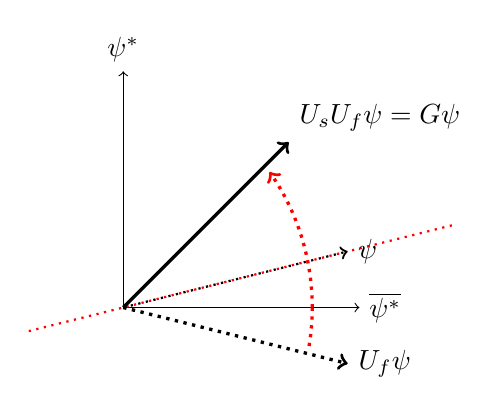
\begin{tikzpicture}[scale=0.6]
            \draw[->] (0,0) -- (5,0) node[anchor=west] {$\ket{\overline{\psi^*}}$};
            \draw[->] (0,0) -- (0,5) node[anchor=south] {$\ket{\psi^*}$};
    
            \draw[very thick, red, dotted, ->] (4,0) arc (0:35:5);
            \draw[very thick, red, dotted] (4,0) arc (0:-10:5);
    
            \draw[thick, red, dotted] (-2, -0.5) -- (7,1.75);
    
            \draw[thick, dotted, ->] (0,0) -- (4.75, 1.1875) node[anchor=west] {$\ket\psi$};
            \draw[very thick, dotted, ->] (0,0) -- (4.75, -1.1875) node[anchor=west] {$U_f\ket\psi$};
    
            \draw[very thick, ->] (0,0) -- (3.5, 3.5) node[anchor=south west] {$U_sU_f\ket\psi = G\ket\psi$};
        \end{tikzpicture}
    }
    \caption{All steps of Grover's algorithm visualized in the plane spanned by all valid configurations $\ket{\psi^*}$ and all non-valid configurations $\ket{\overline{\psi^*}}$}.
    \label{fig:bg:grover:steps}
\end{figure*}

\subsection{Quantum Computing}
\label{sec:bg:qc}
Quantum computing offers a new paradigm in computation, leveraging principles from quantum mechanics such as superposition and entanglement. 
Unlike classical computers, which rely on binary bits, quantum computers use qubits that can exist in multiple states simultaneously. 
While the technology is still in its early stages, it has the potential to provide advantages in specific problem areas like cryptography, optimization, and material science. 
However, it is important to note that quantum computers are not universally faster than classical computers and are best suited to particular types of computational problems.

The fundamental unit of quantum computing is the quantum gate, which is analogous to the classical logic gates utilized in traditional computing and serves as the basic component of a quantum circuit.
These gates facilitate the manipulation of qubits (quantum bits) through operations such as superposition and entanglement. 
It is noteworthy that certain quantum operations can negate one another, such that applying a gate followed by itself has no effect on the qubit's state. 
This property is pivotal for error correction and algorithm design.
Quantum circuits are composed of sequences of these gates, which permit the execution of complex computations through the parallel application of transformations on qubit states.

Two key metrics for assessing the complexity and efficiency of quantum circuits are depth and width.
\begin{description}
    \item[Width] The width of a quantum circuit is defined as the number of qubits utilized, and it determines the amount of information that the circuit can process in parallel.
    \item[Depth] The depth of a quantum circuit is a measure of the number of layers of gates applied sequentially.
    It is a reflection of the length of time required for the computation, as each layer can be executed simultaneously. 
\end{description}
A circuit with greater depth requires more time to execute, whereas a circuit with greater width can accommodate more complex states or parallel operations. 
The interplay between depth and width is crucial for understanding the resource requirements and potential limitations of quantum algorithms.

\subsection{Quantum Programming}
Qiskit is a widely used open-source quantum computing framework developed by IBM \cite{Qiskit}, designed to enable the creation, simulation, and execution of quantum circuits on both simulators and real quantum hardware. 
It provides a high-level Python interface for designing quantum algorithms, optimizing quantum circuits, and performing tasks such as quantum error correction, gate decomposition, and circuit transpilation. 
One of its core strengths is its ability to transpile circuits to match the constraints of actual quantum processors, such as gate set compatibility and qubit connectivity. 
This makes it highly versatile for both research and practical applications in quantum computing.

Complementing Qiskit is Quantum Assembly Language (QASM) \cite{cross2017openquantumassemblylanguage} \cite{OpenQASM3.0}, a low-level, hardware-agnostic language used to describe quantum circuits as a series of quantum gate operations and measurements.
QASM serves as the interface between high-level quantum algorithms and quantum hardware, translating the abstract structure of quantum circuits into executable instructions. 
This combination of Qiskit’s high-level capabilities and QASM’s precise control over quantum operations enables researchers and developers to experiment with quantum algorithms on various platforms, ranging from simulators to quantum hardware.

\subsection{Grover's Algorithm}
One of the most notable quantum algorithms is Grover's algorithm. 
Published by L. K. Grover in 1996 \cite{grover1996}, it exemplifies the power of quantum circuits by markedly accelerating the search process in unsorted databases, offering a quadratic speedup compared to classical algorithms. 
As searching solutions to logical formulae can be translated into finding possible solutions to the formula in a database containing all possible variable assignments, it can be seen that Grover's algorithm can also be used to solve logical formulae.
Grover can be mainly divided into three important steps

\begin{enumerate}
    \item \textbf{Preparation:} Prepares all $n$ non-ancilla qubits into a superposition state $\ket\psi$ consisting of $2^n$ possible states. In the context of Software Product Lines, $n$ describes the amount of features.
    \item \textbf{Oracle:} Marks all states that are valid solutions of our problem by negating their phase. In our context this means to mark all states that are valid configurations of our feature model. In a mathematical context this means to multiply our state $\ket\psi$ by the oracle operator/matrix $U_f$ resulting in our temporary state $U_f\ket\psi$.
    \item \textbf{Diffusion:} In the final step of Grover's algorithm we take the state $U_f\ket\psi$ and reflect it about the prepared state $\ket\psi$. Mathematically this means we multiply by another operation matrix $U_s$, giving us the state $U_sU_f\ket\psi$.
\end{enumerate}

This process is visualized in Figure \ref{fig:bg:grover:steps}. It displays the current state of our quantum system as a bold arrow in the plane of all possible $2^n$ configurations.
This plane is spanned by the two states $\ket{\psi^*}$ which describes a state consisting only of \textit{valid} configurations of our feature model, and state $\ket{\overline{\psi^*}}$ which consists of all \textit{invalid} configurations.
The last two steps, namely \textit{Oracle} ($U_f$) and \textit{Diffusion} ($U_s$) together are also called a \textit{Grover iteration} ($U_sU_f$).
This Grover iteration has to be repeated for  $\sim\frac{\pi}{4}\sqrt{N/M}$ solutions, where $N=2^n$ is the number of all \textit{possible} configurations, while $M$ describes all \textit{valid} configurations.

